% Created 2019-04-27 Sat 21:05
\documentclass[11pt]{article}
\usepackage[utf8]{inputenc}
\usepackage[T1]{fontenc}
\usepackage{fixltx2e}
\usepackage{graphicx}
\usepackage{longtable}
\usepackage{float}
\usepackage{wrapfig}
\usepackage{rotating}
\usepackage[normalem]{ulem}
\usepackage{amsmath}
\usepackage{textcomp}
\usepackage{marvosym}
\usepackage{wasysym}
\usepackage{amssymb}
\usepackage{hyperref}
\tolerance=1000
\author{Jonatan Ahumada Fernández}
\date{\today}
\title{Taller: graffitis}
\hypersetup{
  pdfkeywords={},
  pdfsubject={},
  pdfcreator={Emacs 25.3.50.1 (Org mode 8.2.10)}}
\begin{document}

\maketitle
\tableofcontents

\begin{center}
\begin{tabular}{llll}
\hline
Street Art & Desc. & Graffiti & Desc.\\
\hline
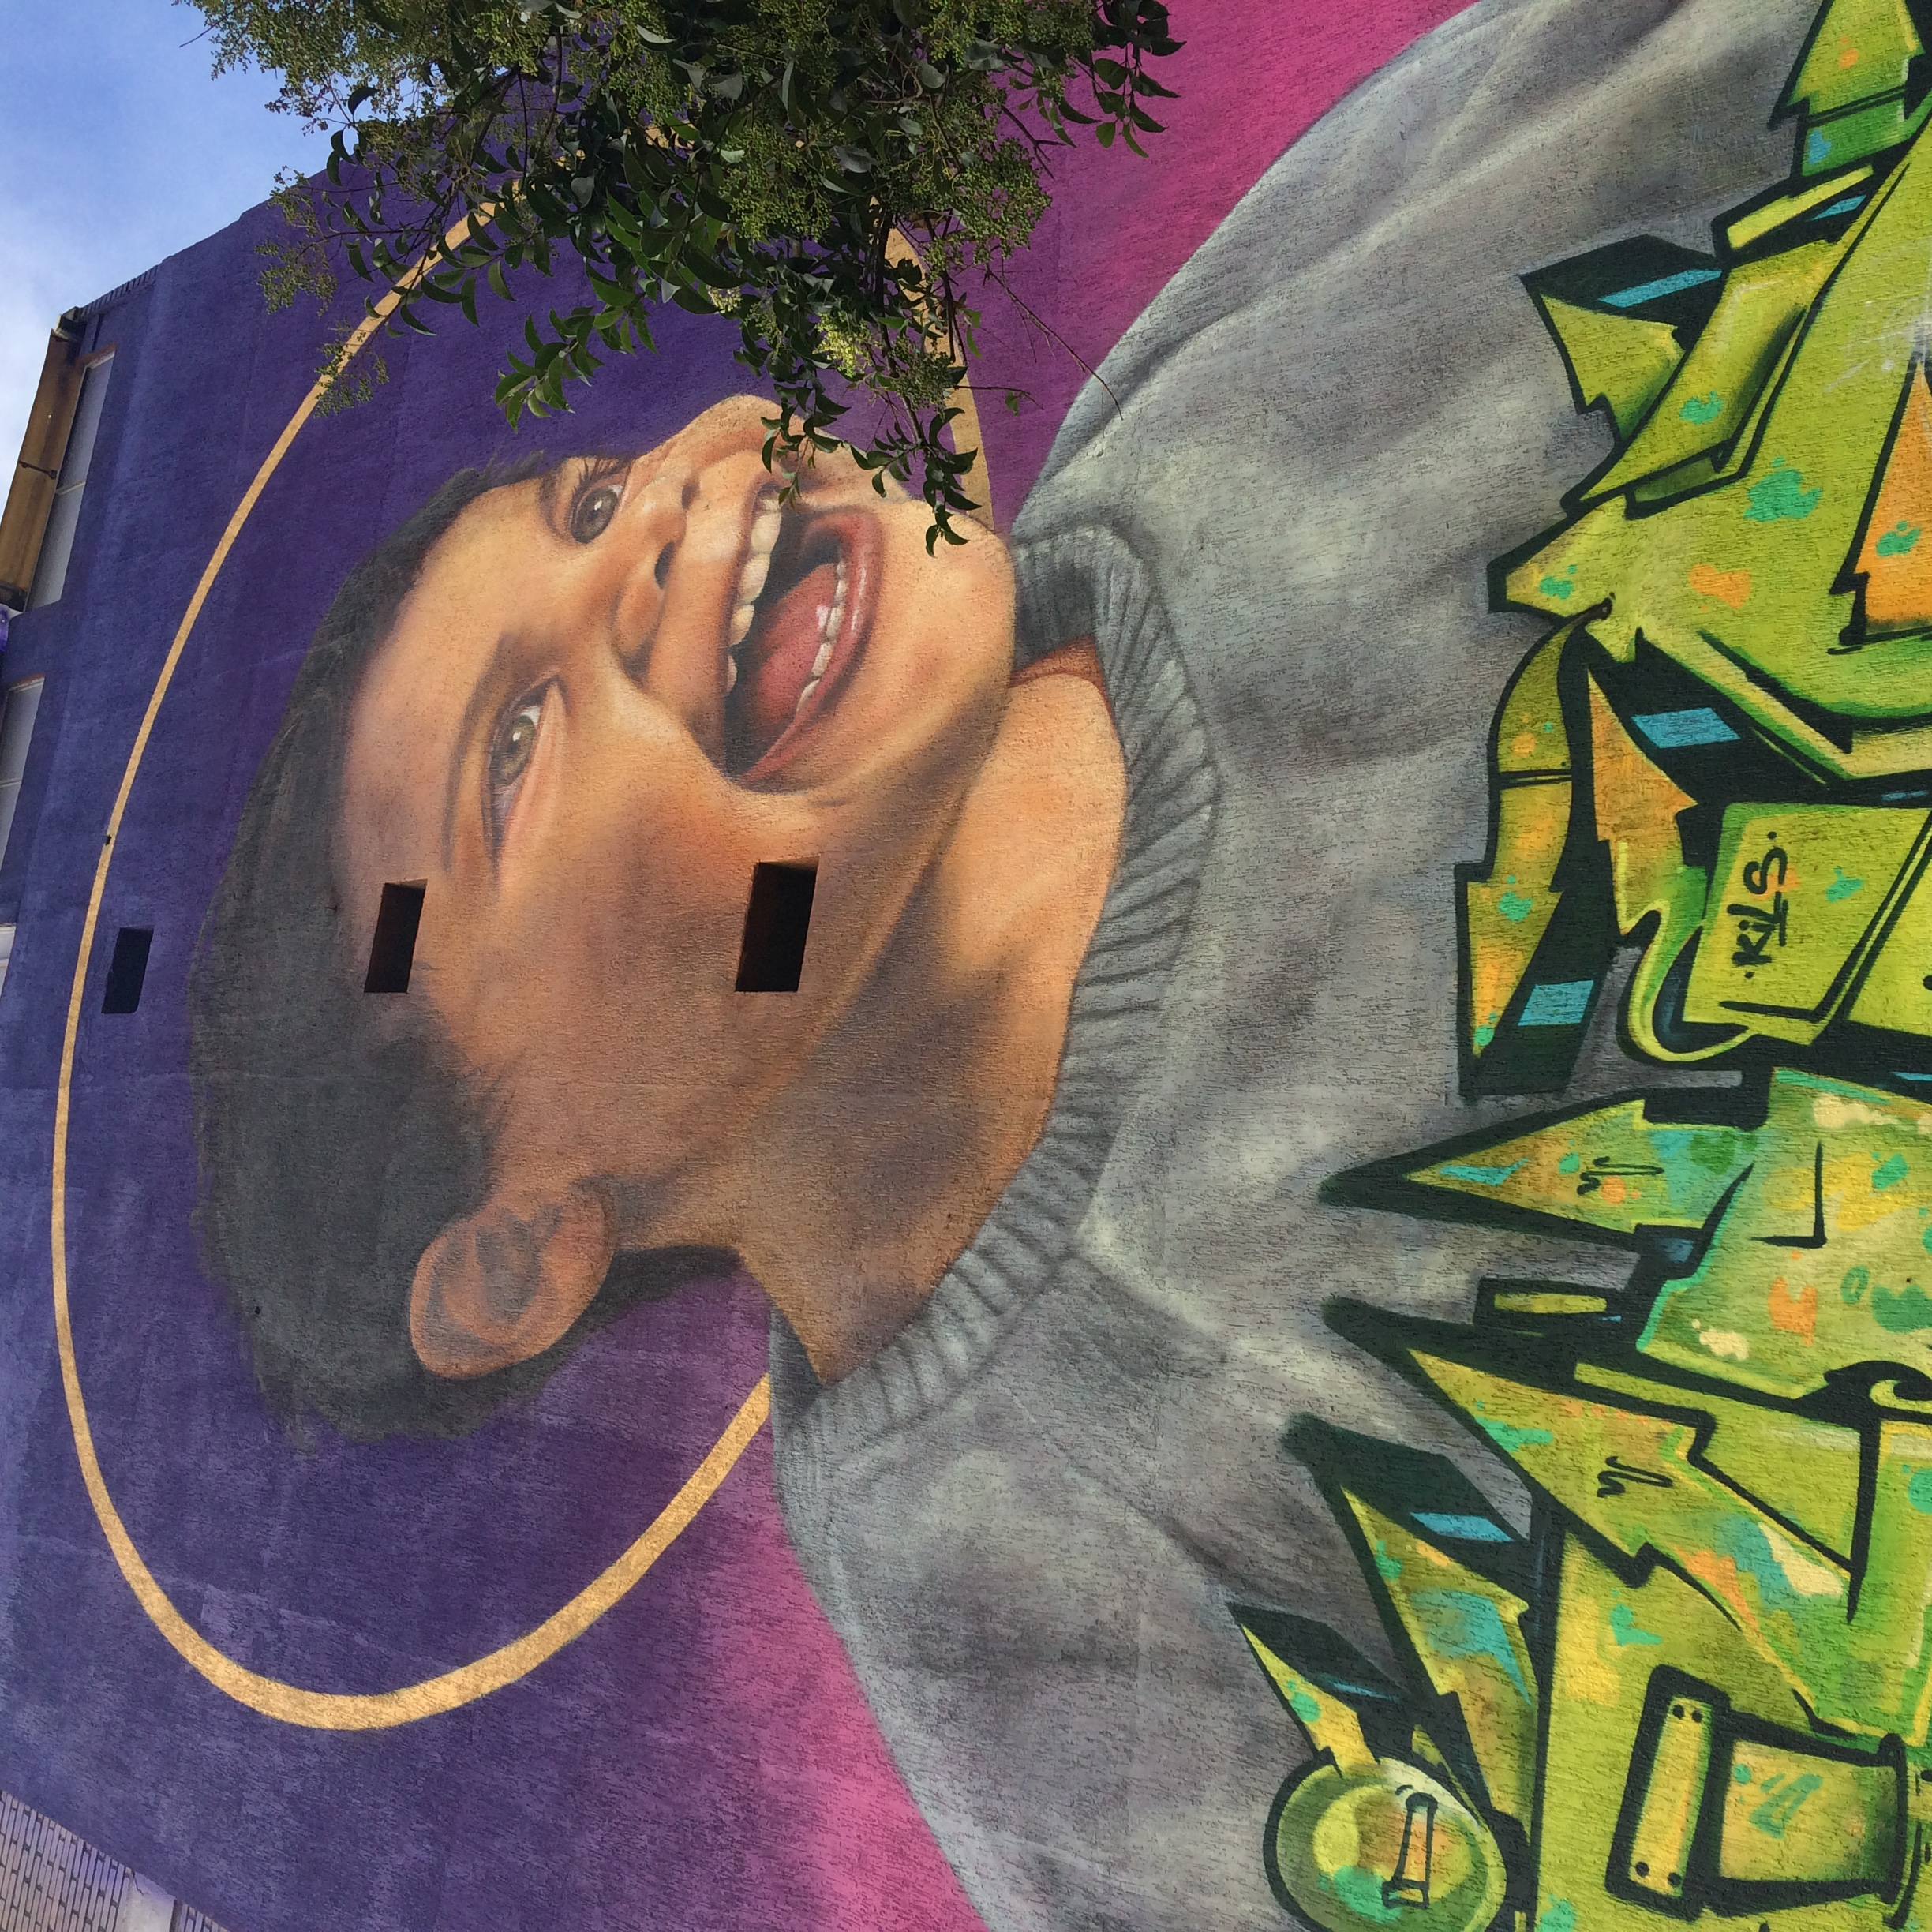
\includegraphics[width=.9\linewidth]{./graffitti/ninio.JPG} & - complejidad + materiales & 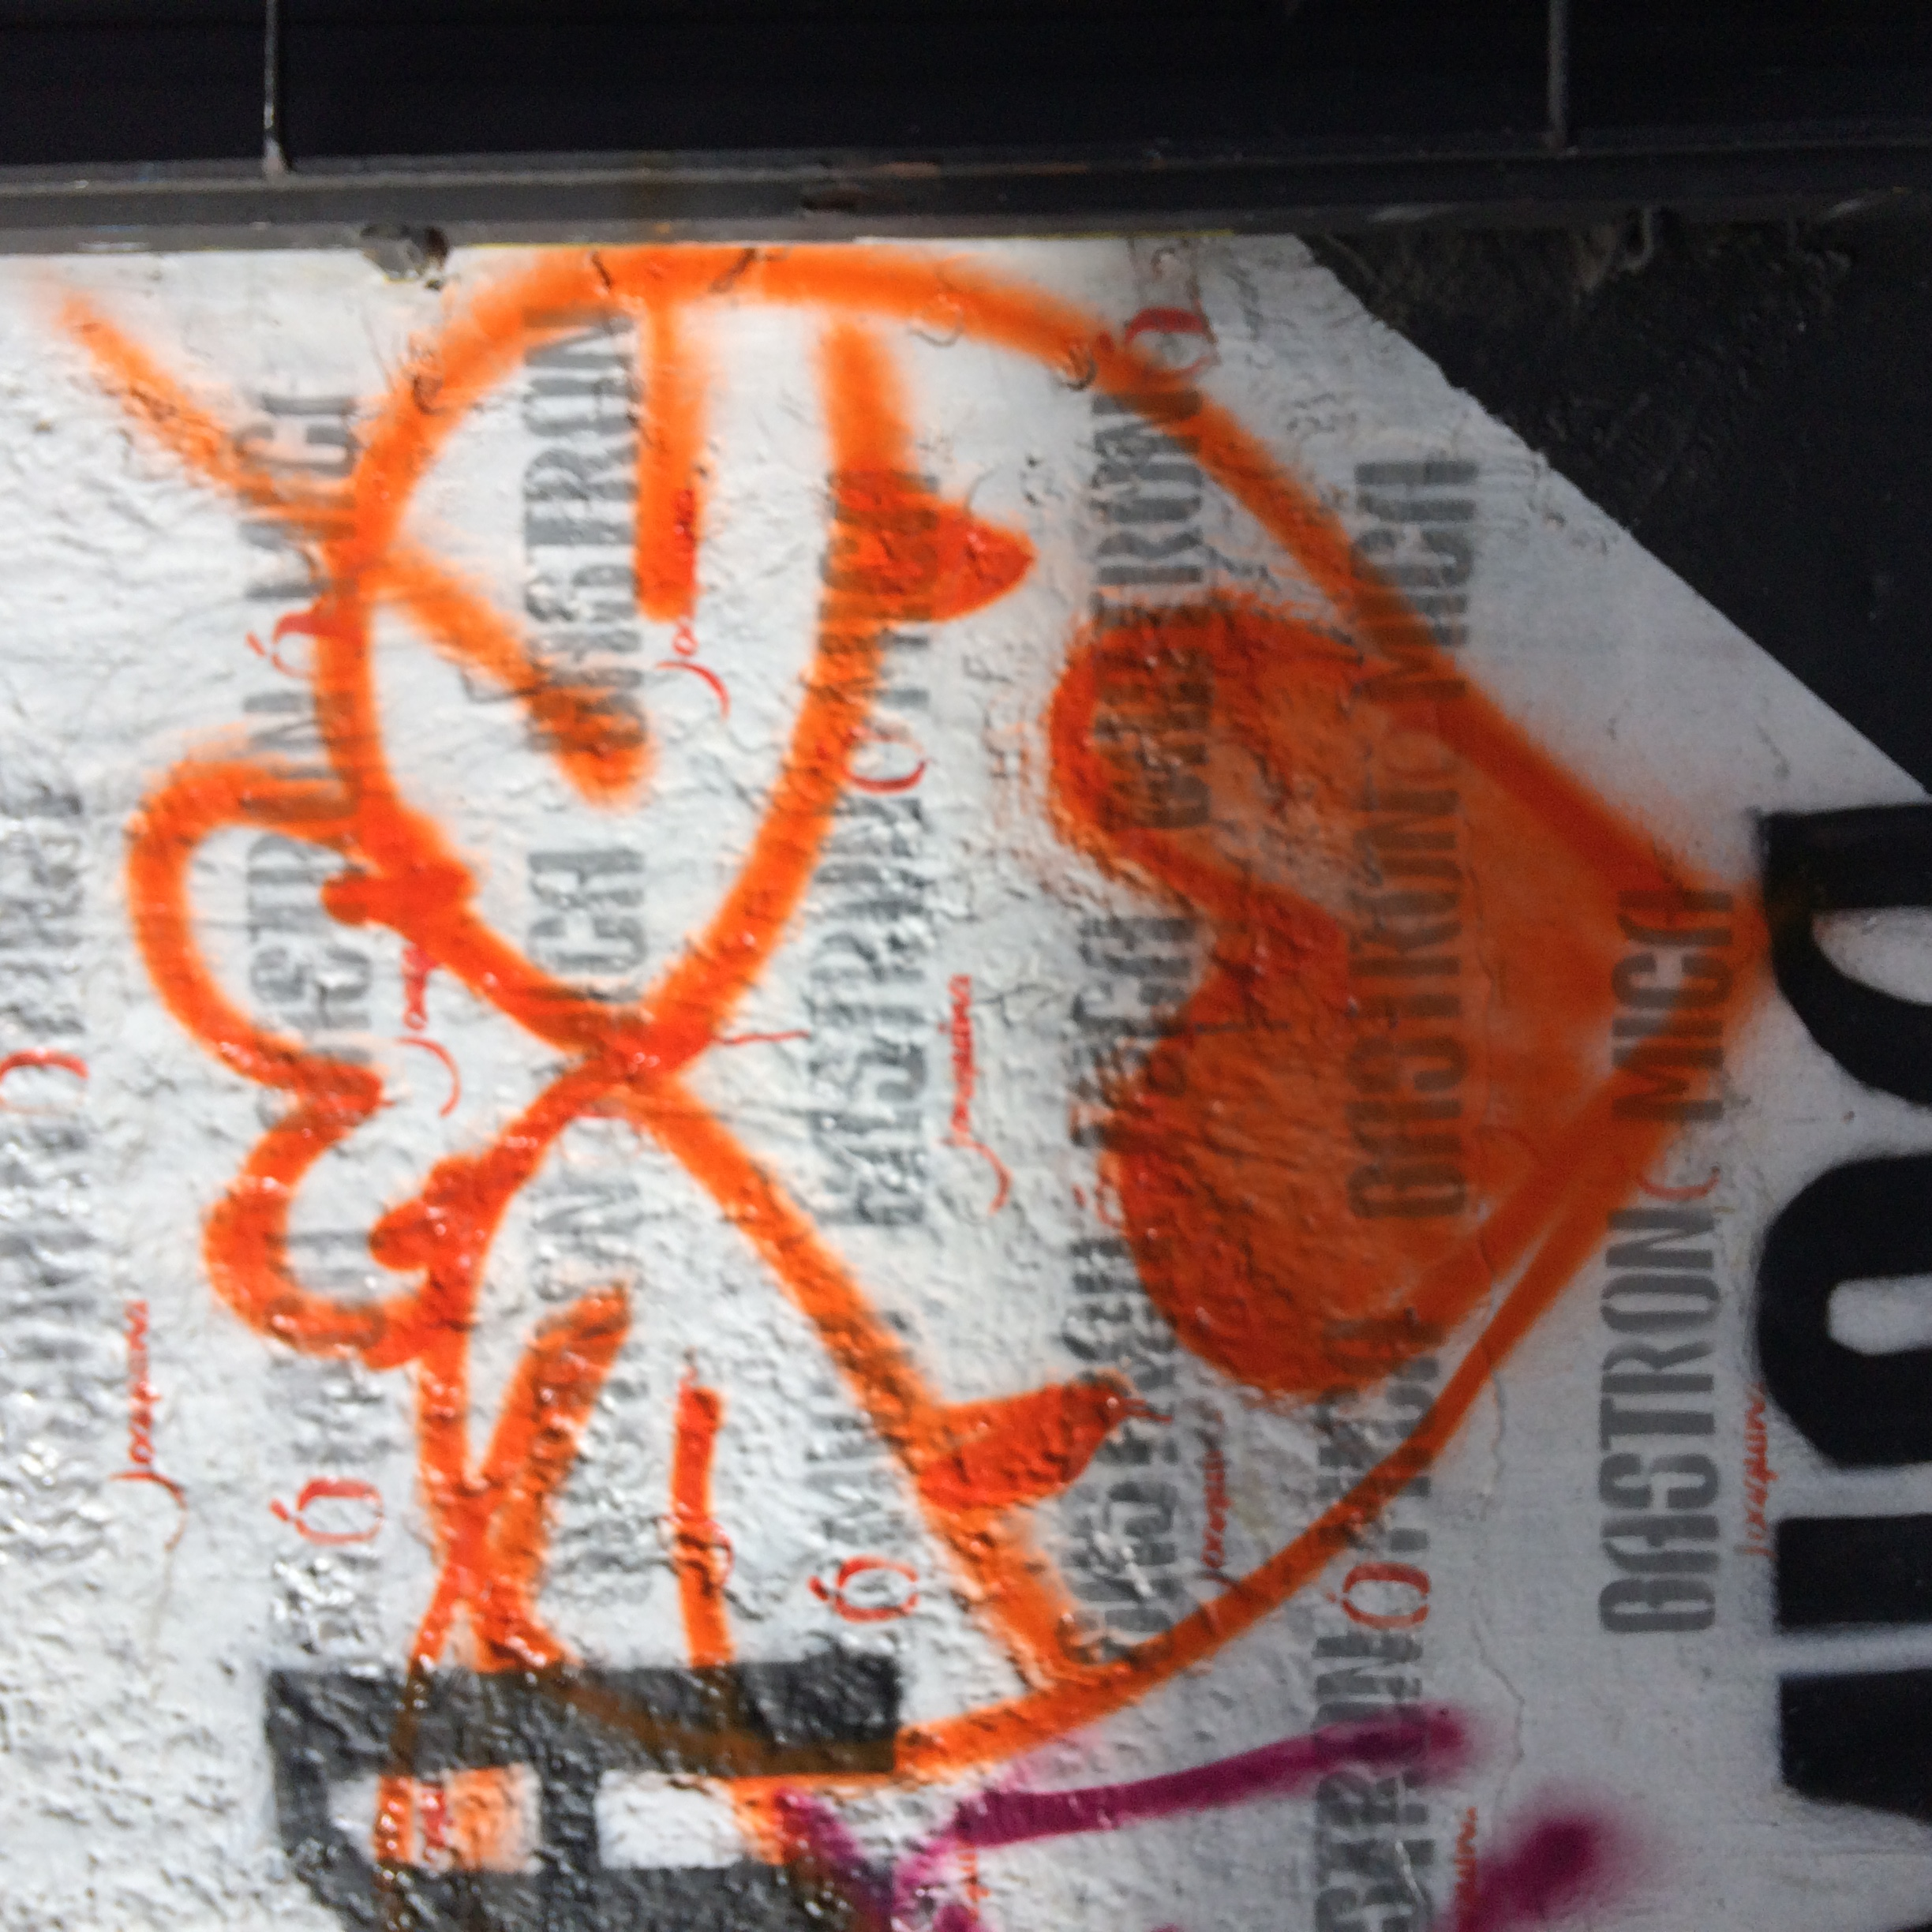
\includegraphics[width=.9\linewidth]{./graffitti/gffti1.JPG} & \\
 & - probablemente un colectivo &  & \\
 & - &  & \\
\hline
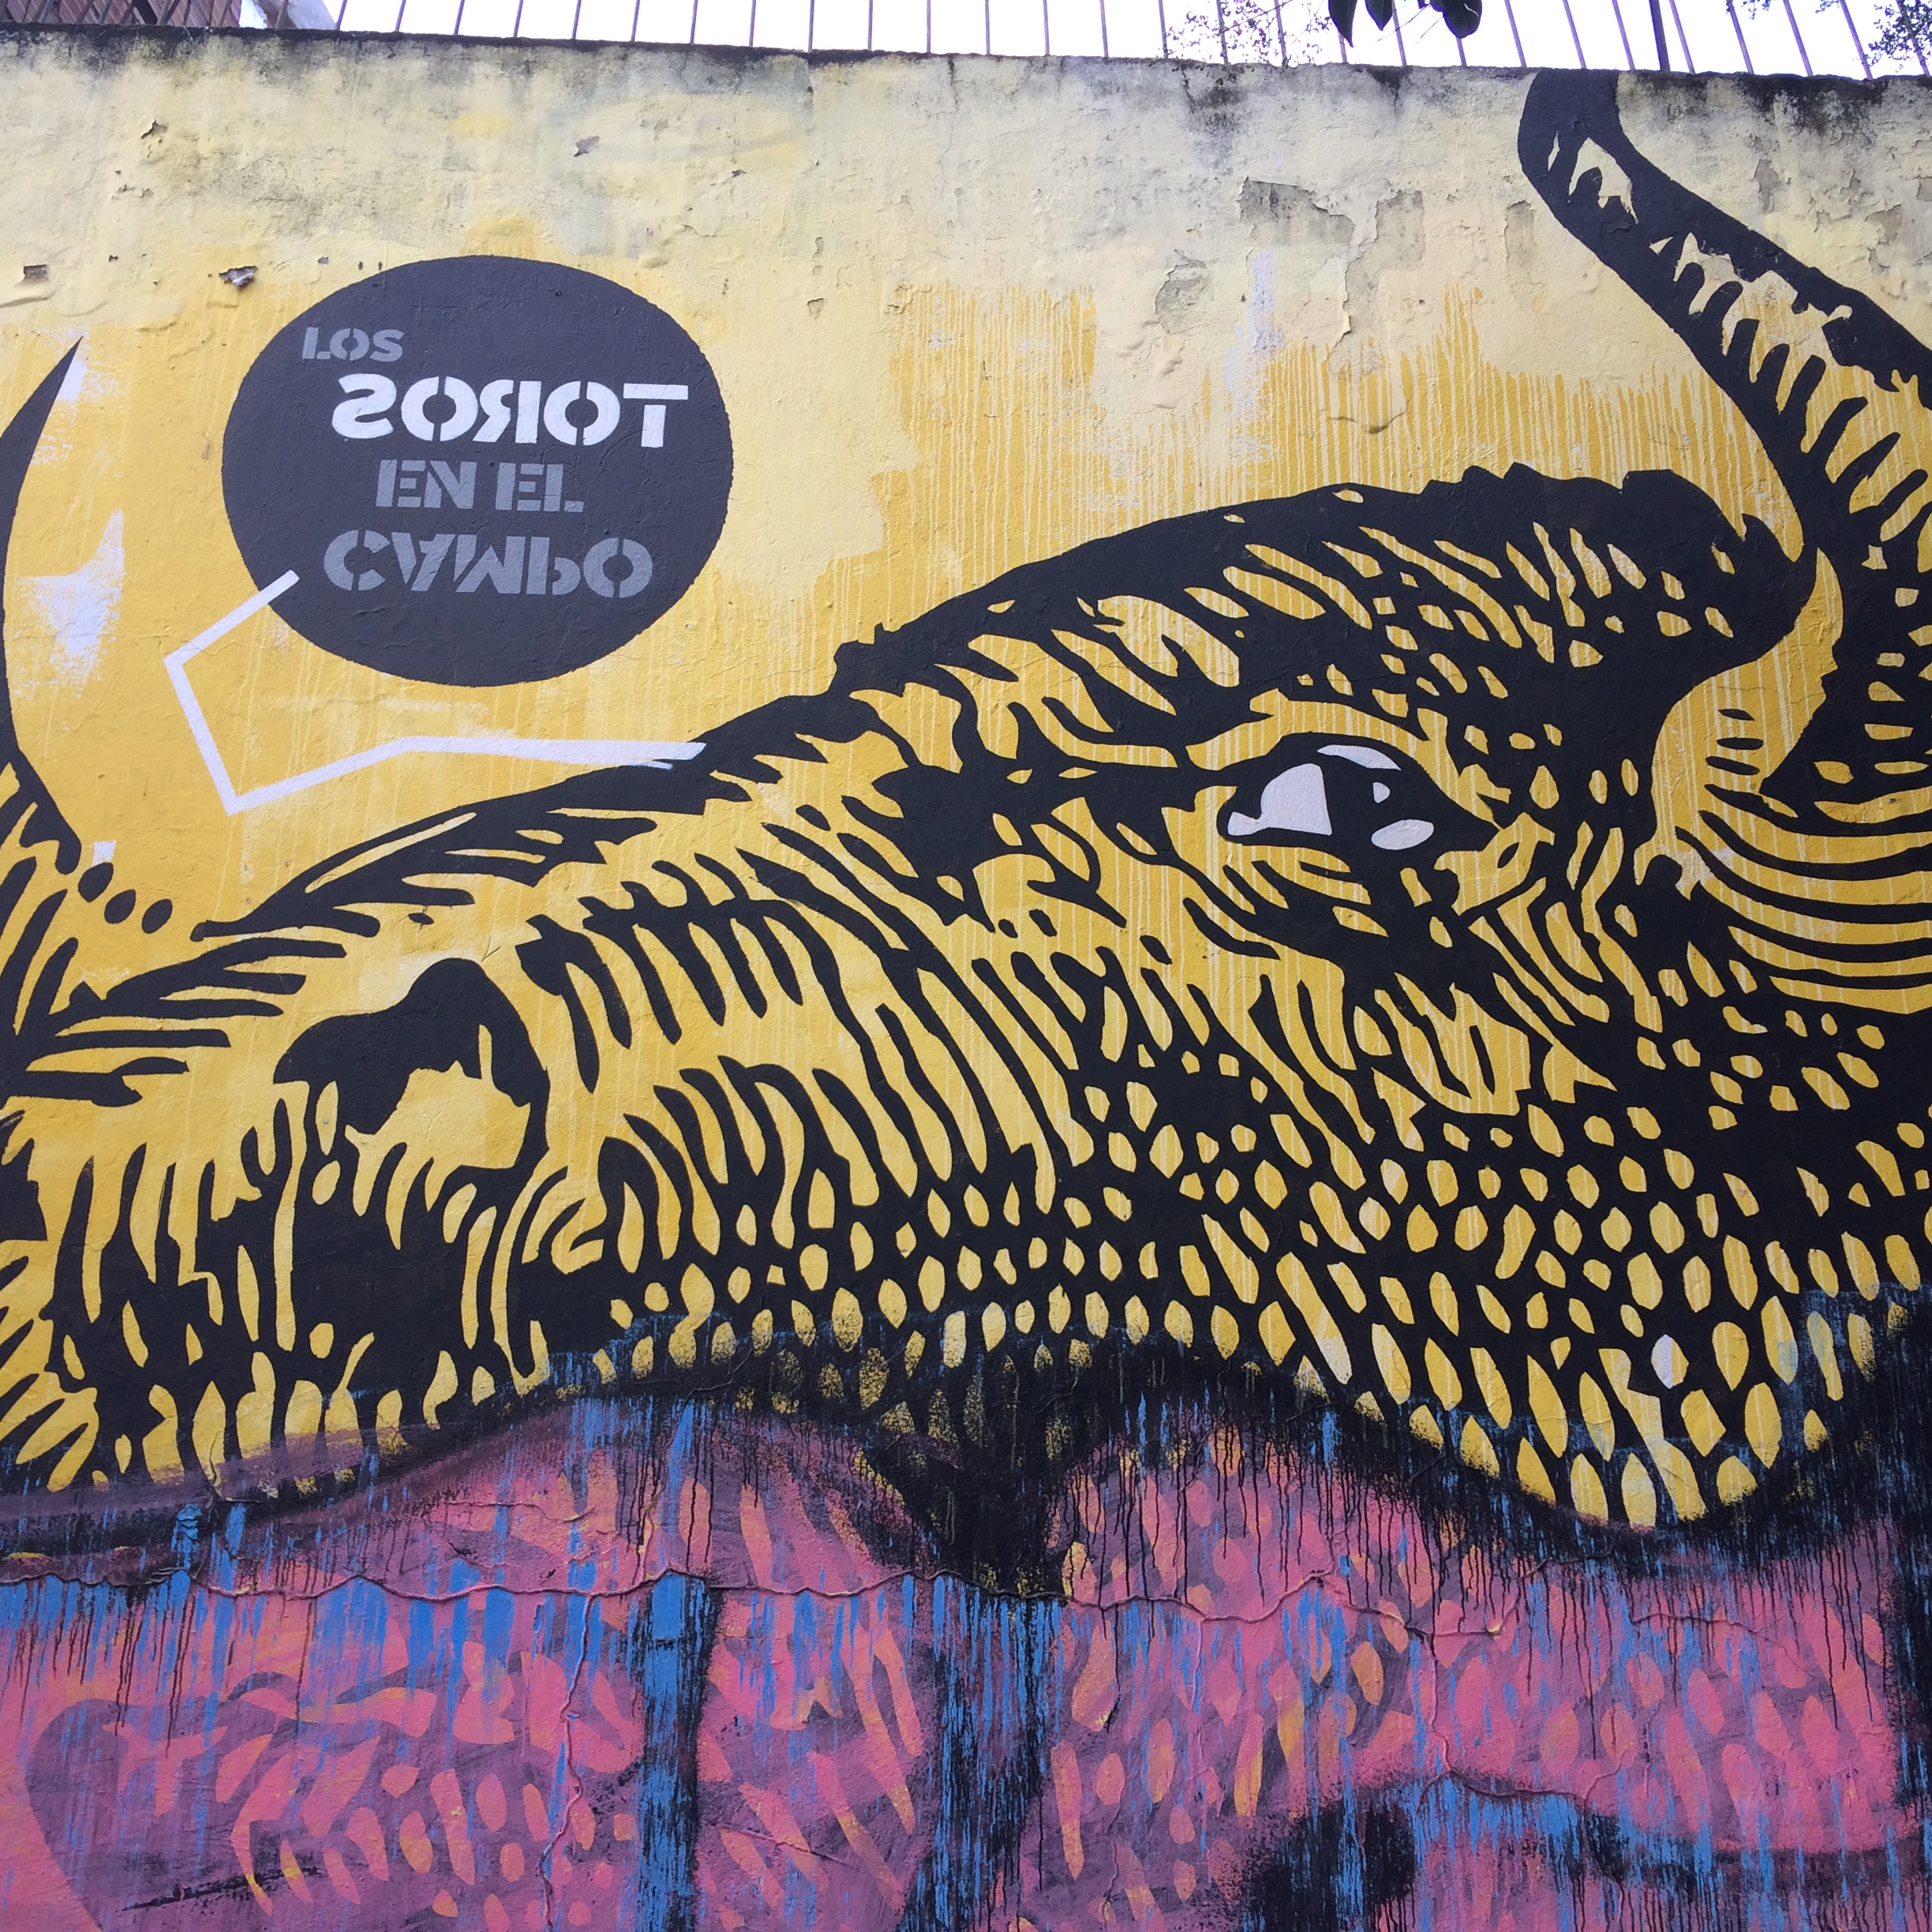
\includegraphics[width=.9\linewidth]{./graffitti/toro.JPG} & - usa stencil & 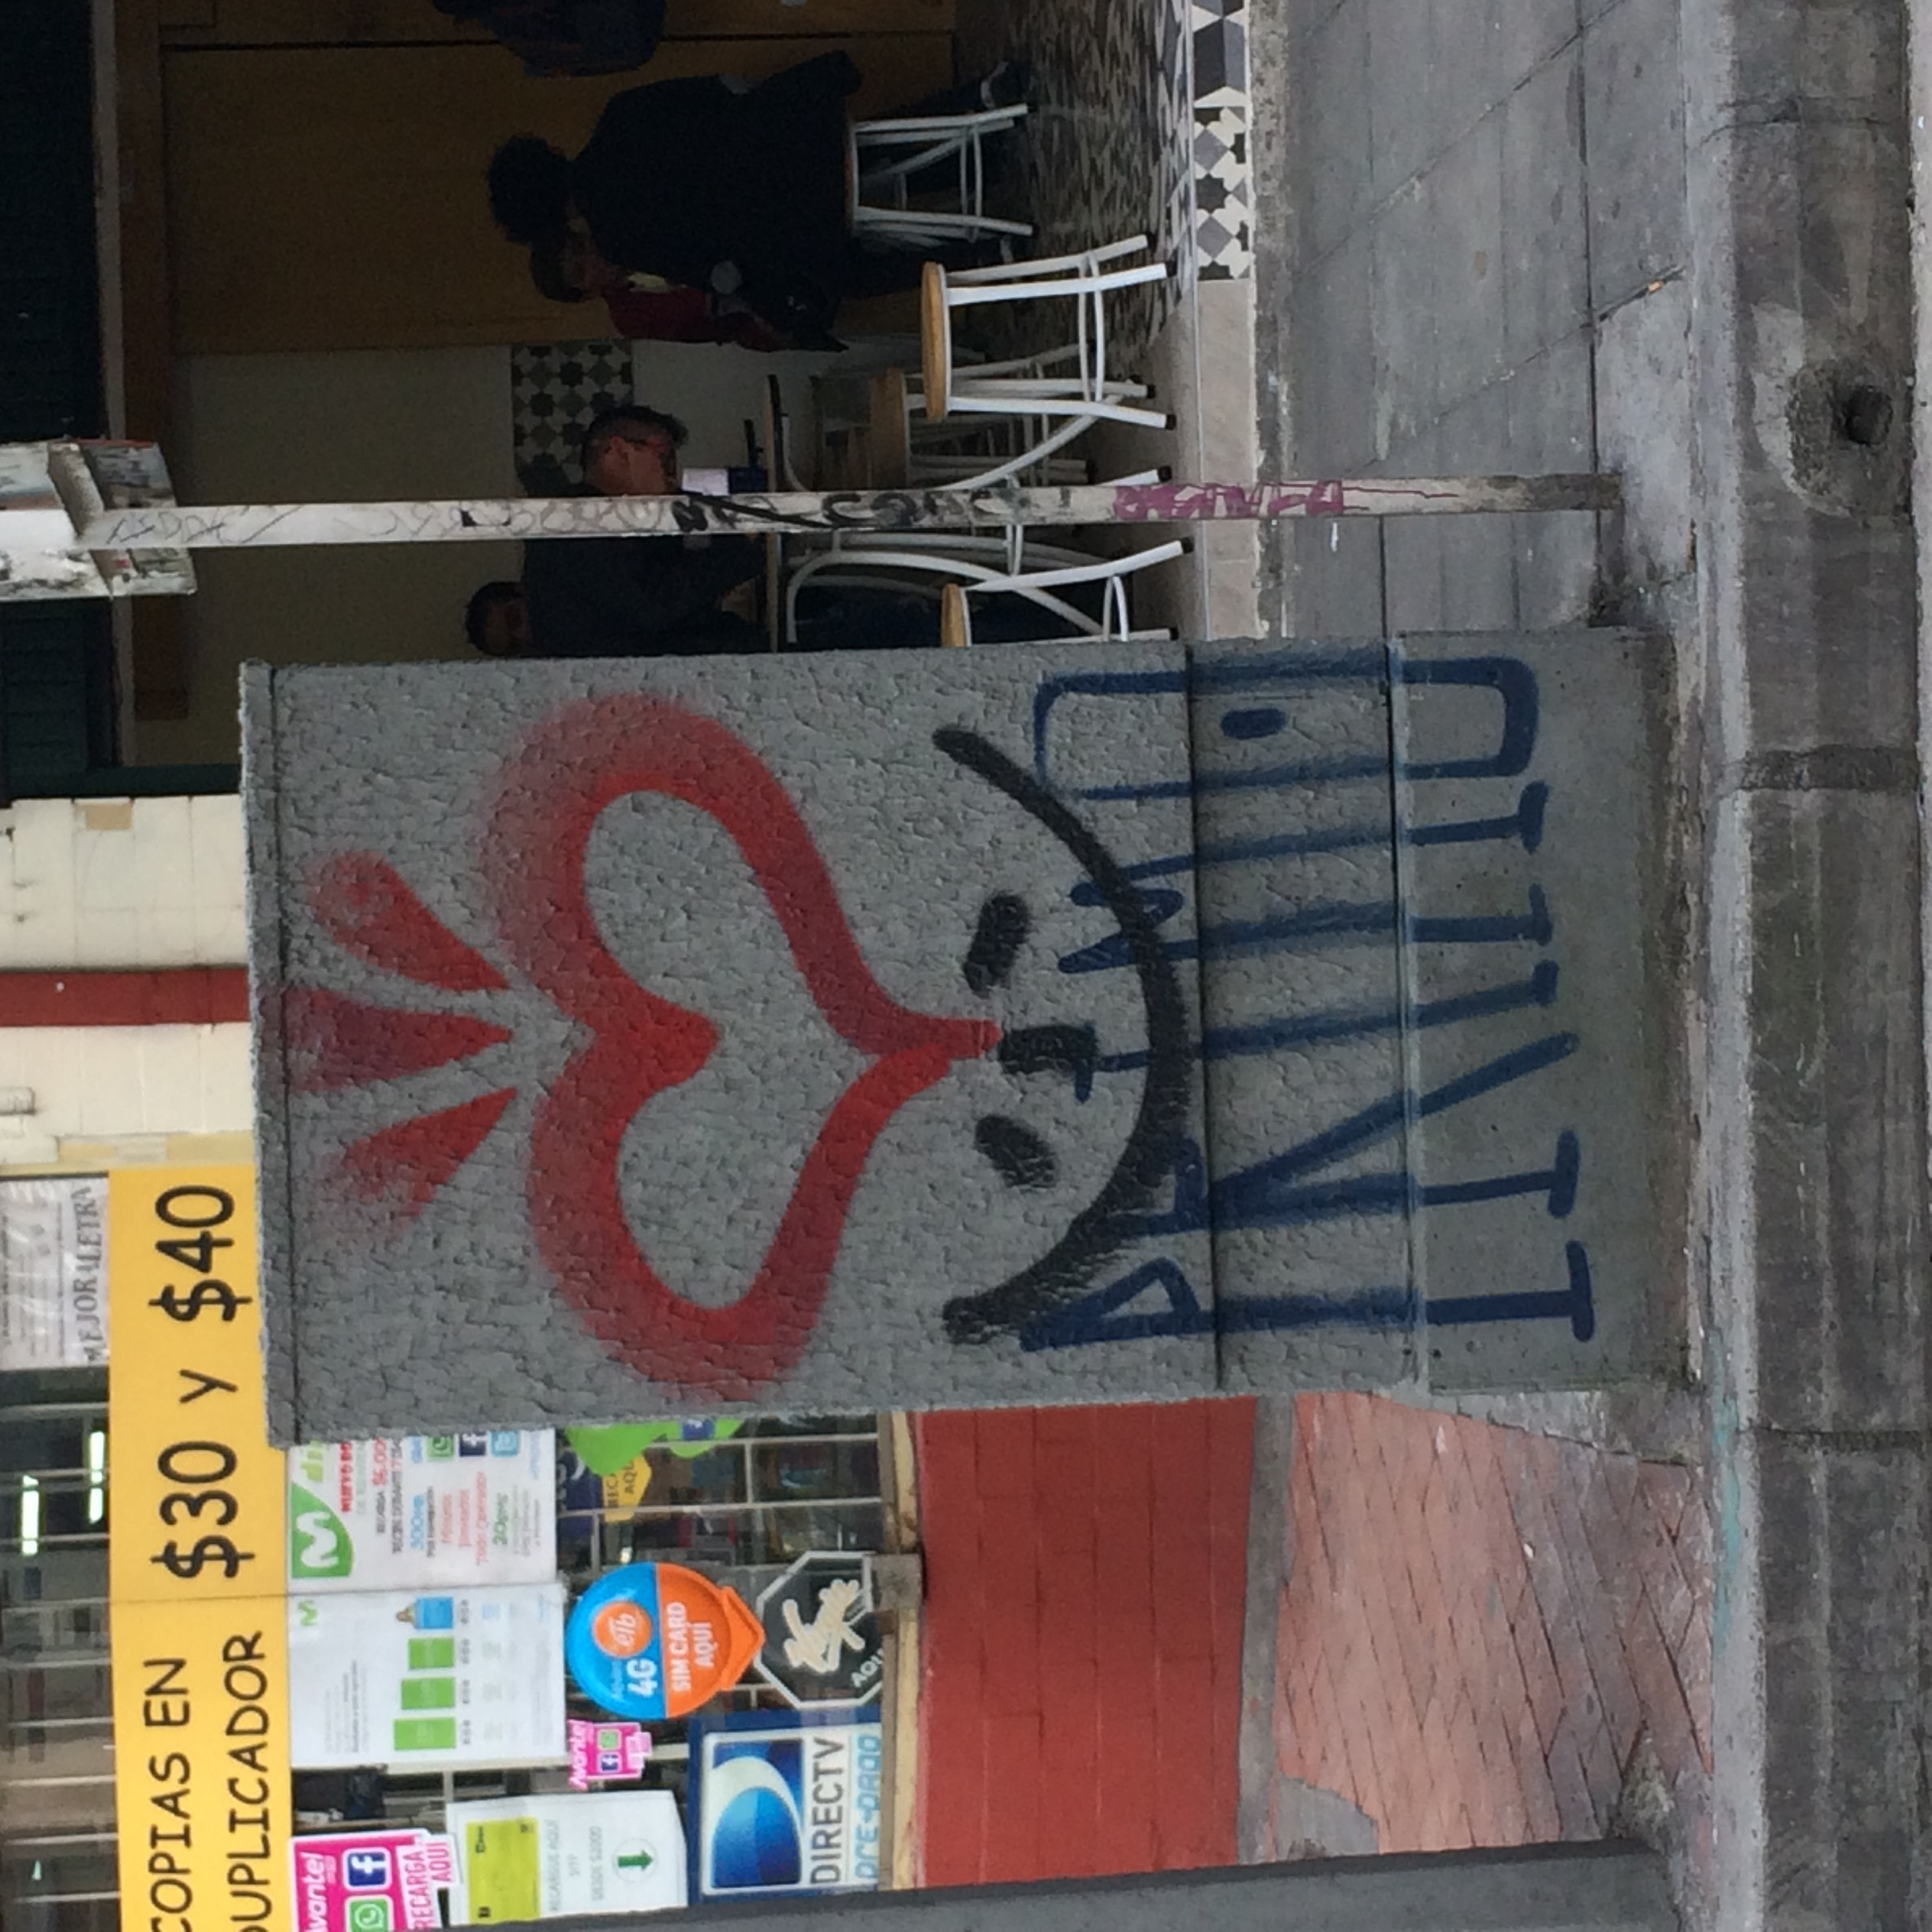
\includegraphics[width=.9\linewidth]{./graffitti/gffti2.JPG} & \\
 & - nombre del colectivo &  & \\
\hline
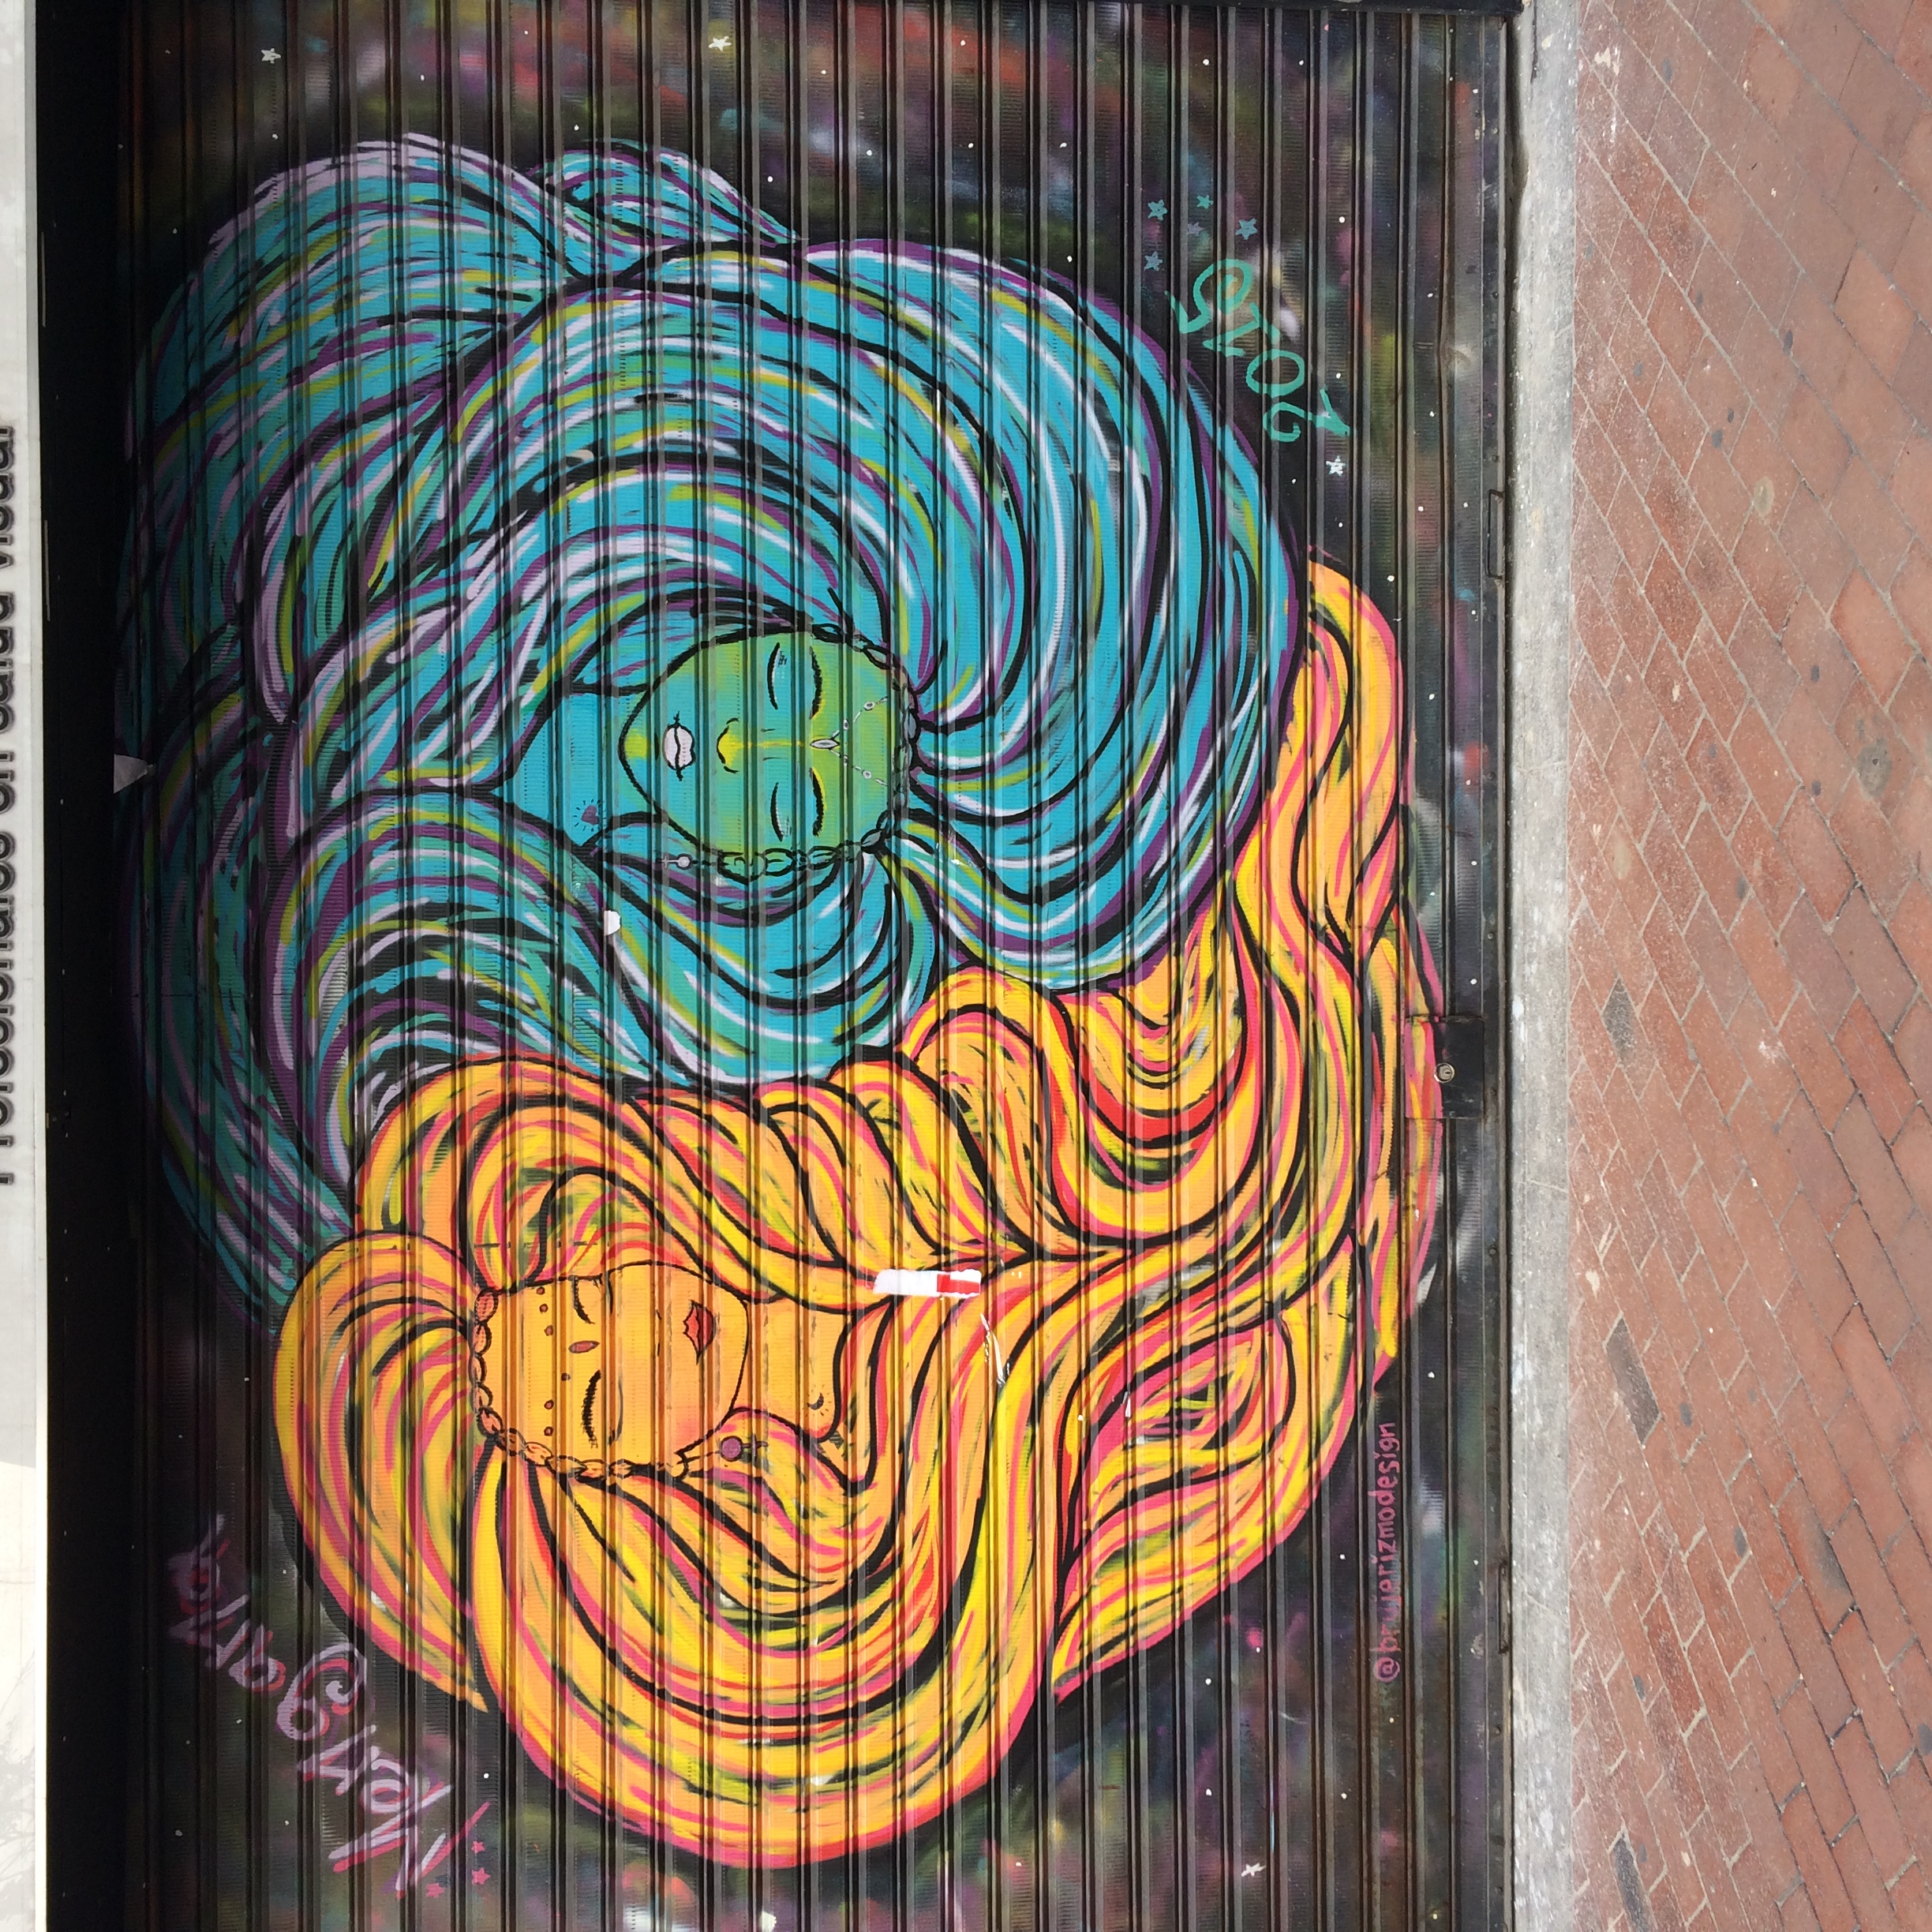
\includegraphics[width=.9\linewidth]{./graffiti/mujeres.JPG} & - composición (ying/yang) & 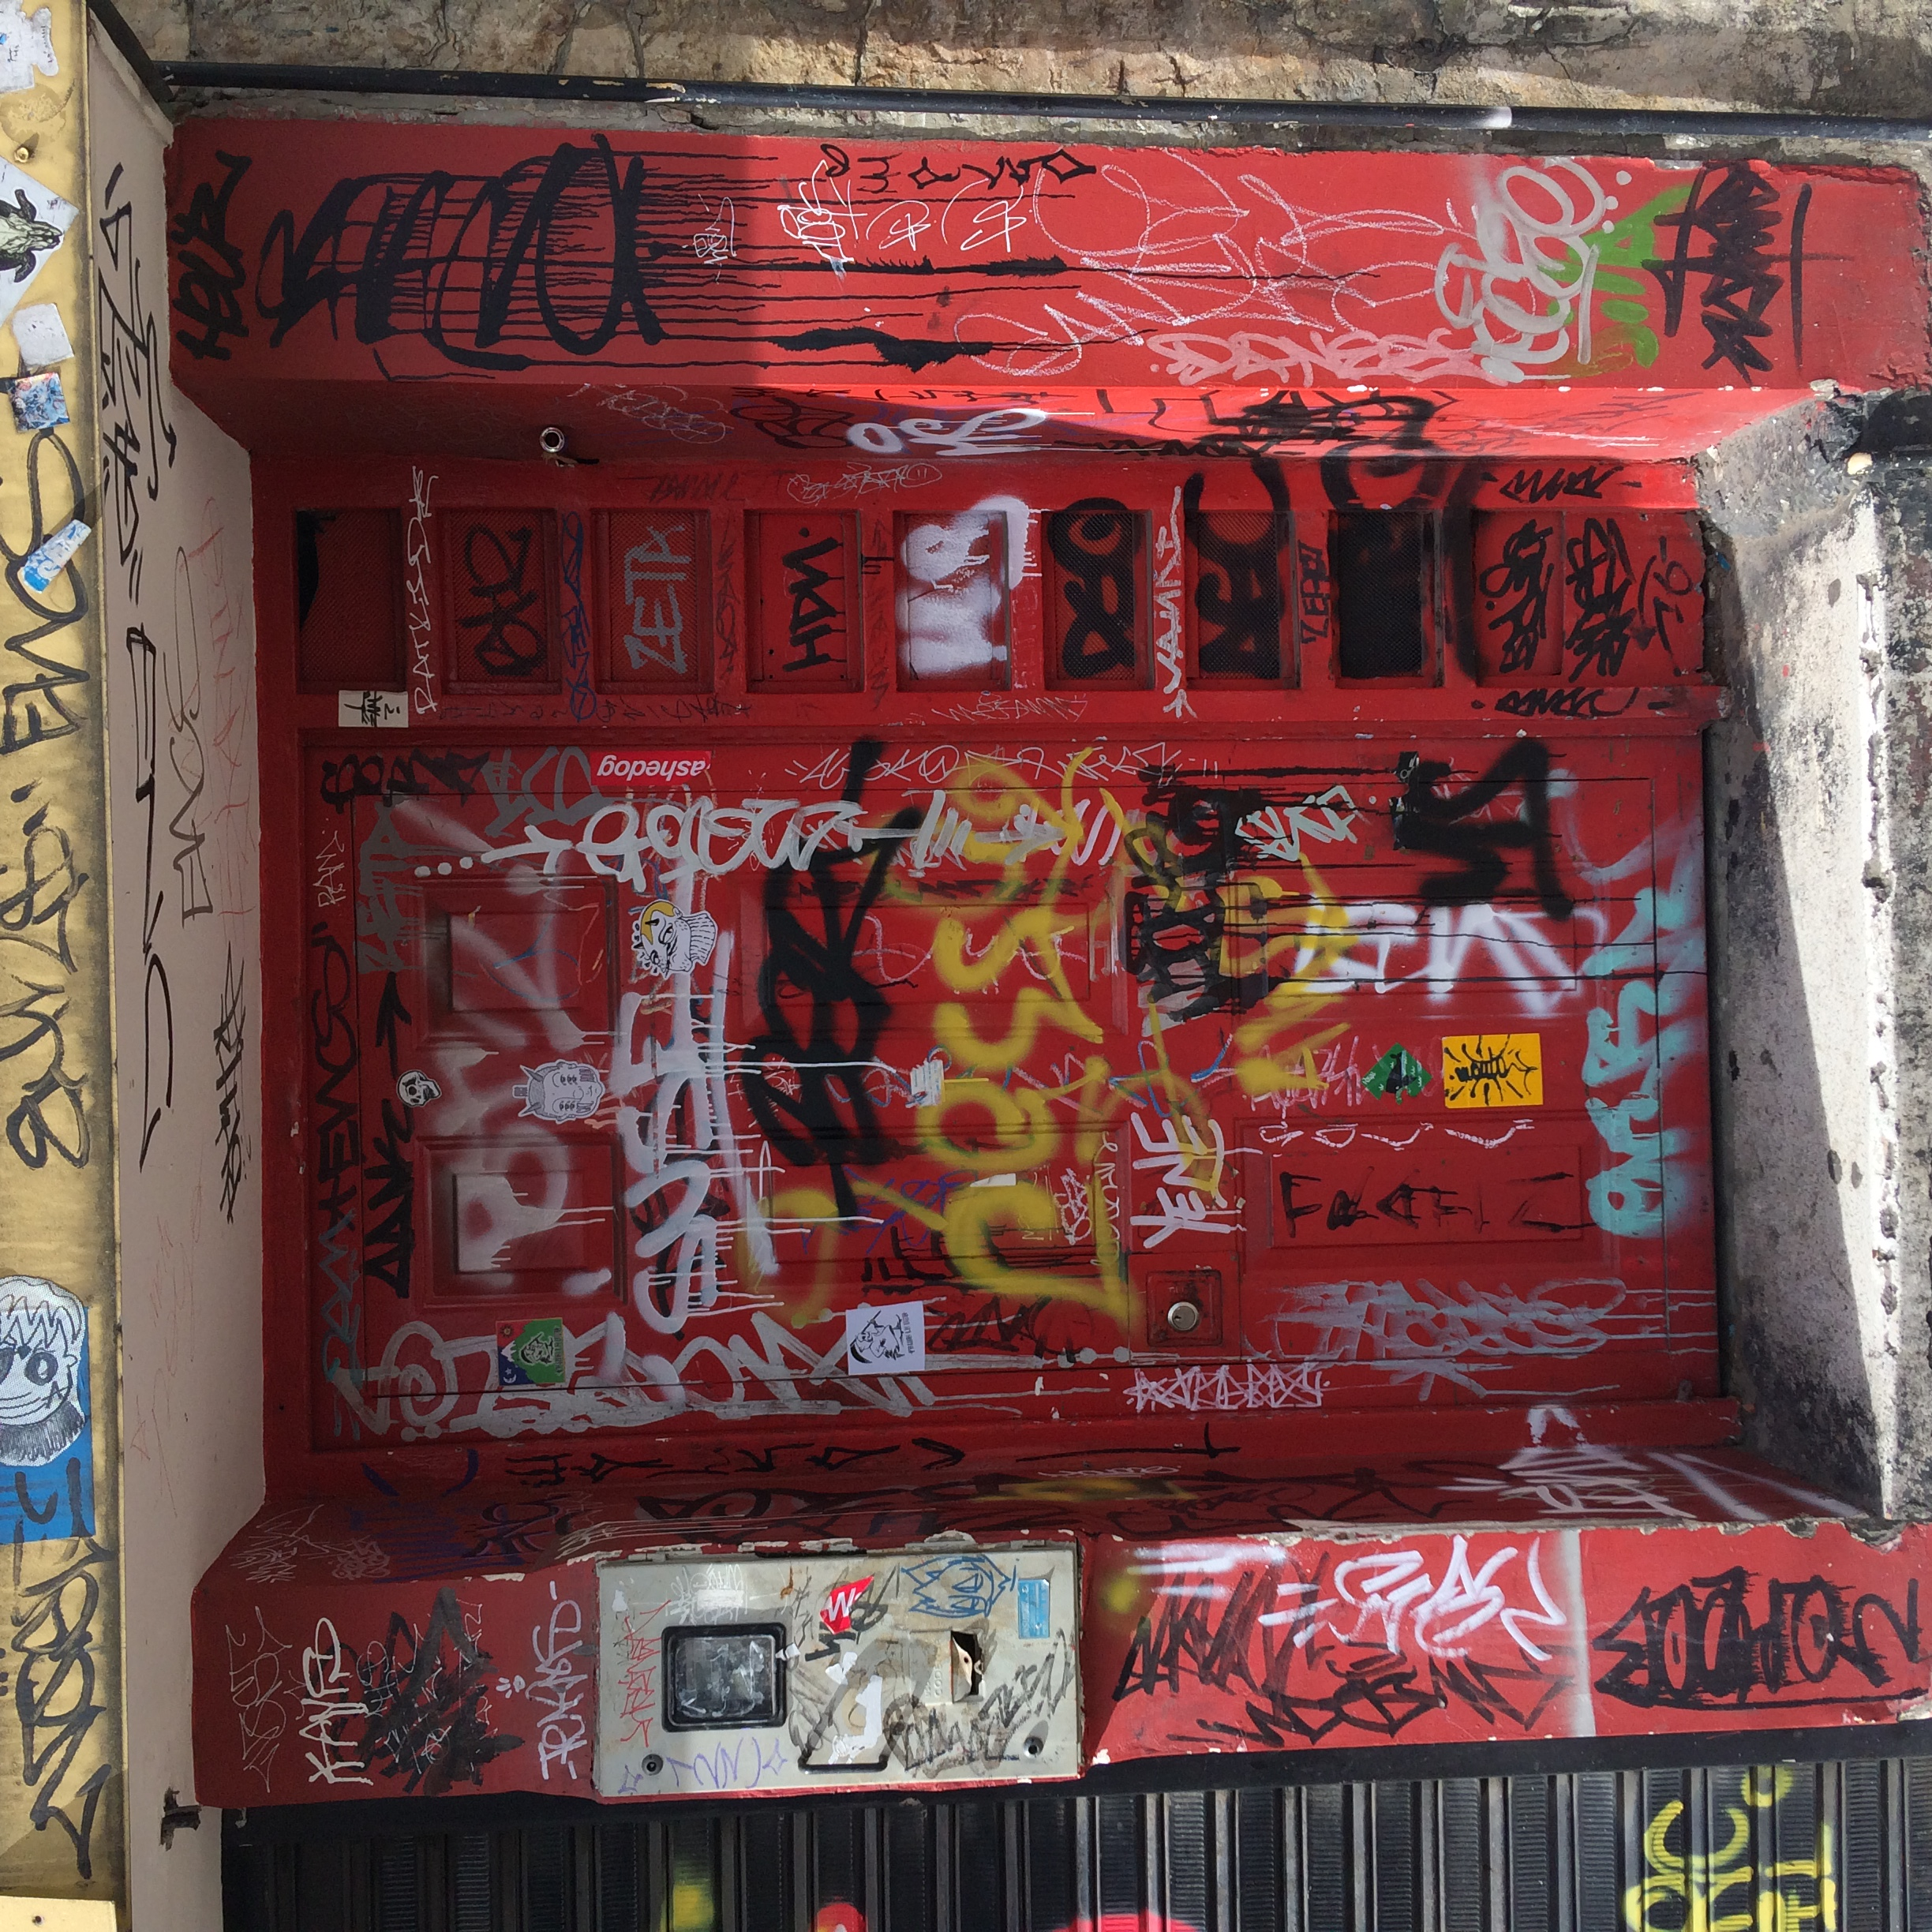
\includegraphics[width=.9\linewidth]{./graffitti/gffti3.JPG} & \\
 & - mensaje femenista &  & \\
 & - colectivo de modas &  & \\
 & - @brujerismodesign &  & \\
 & - no hay anonimidad &  & \\
\hline
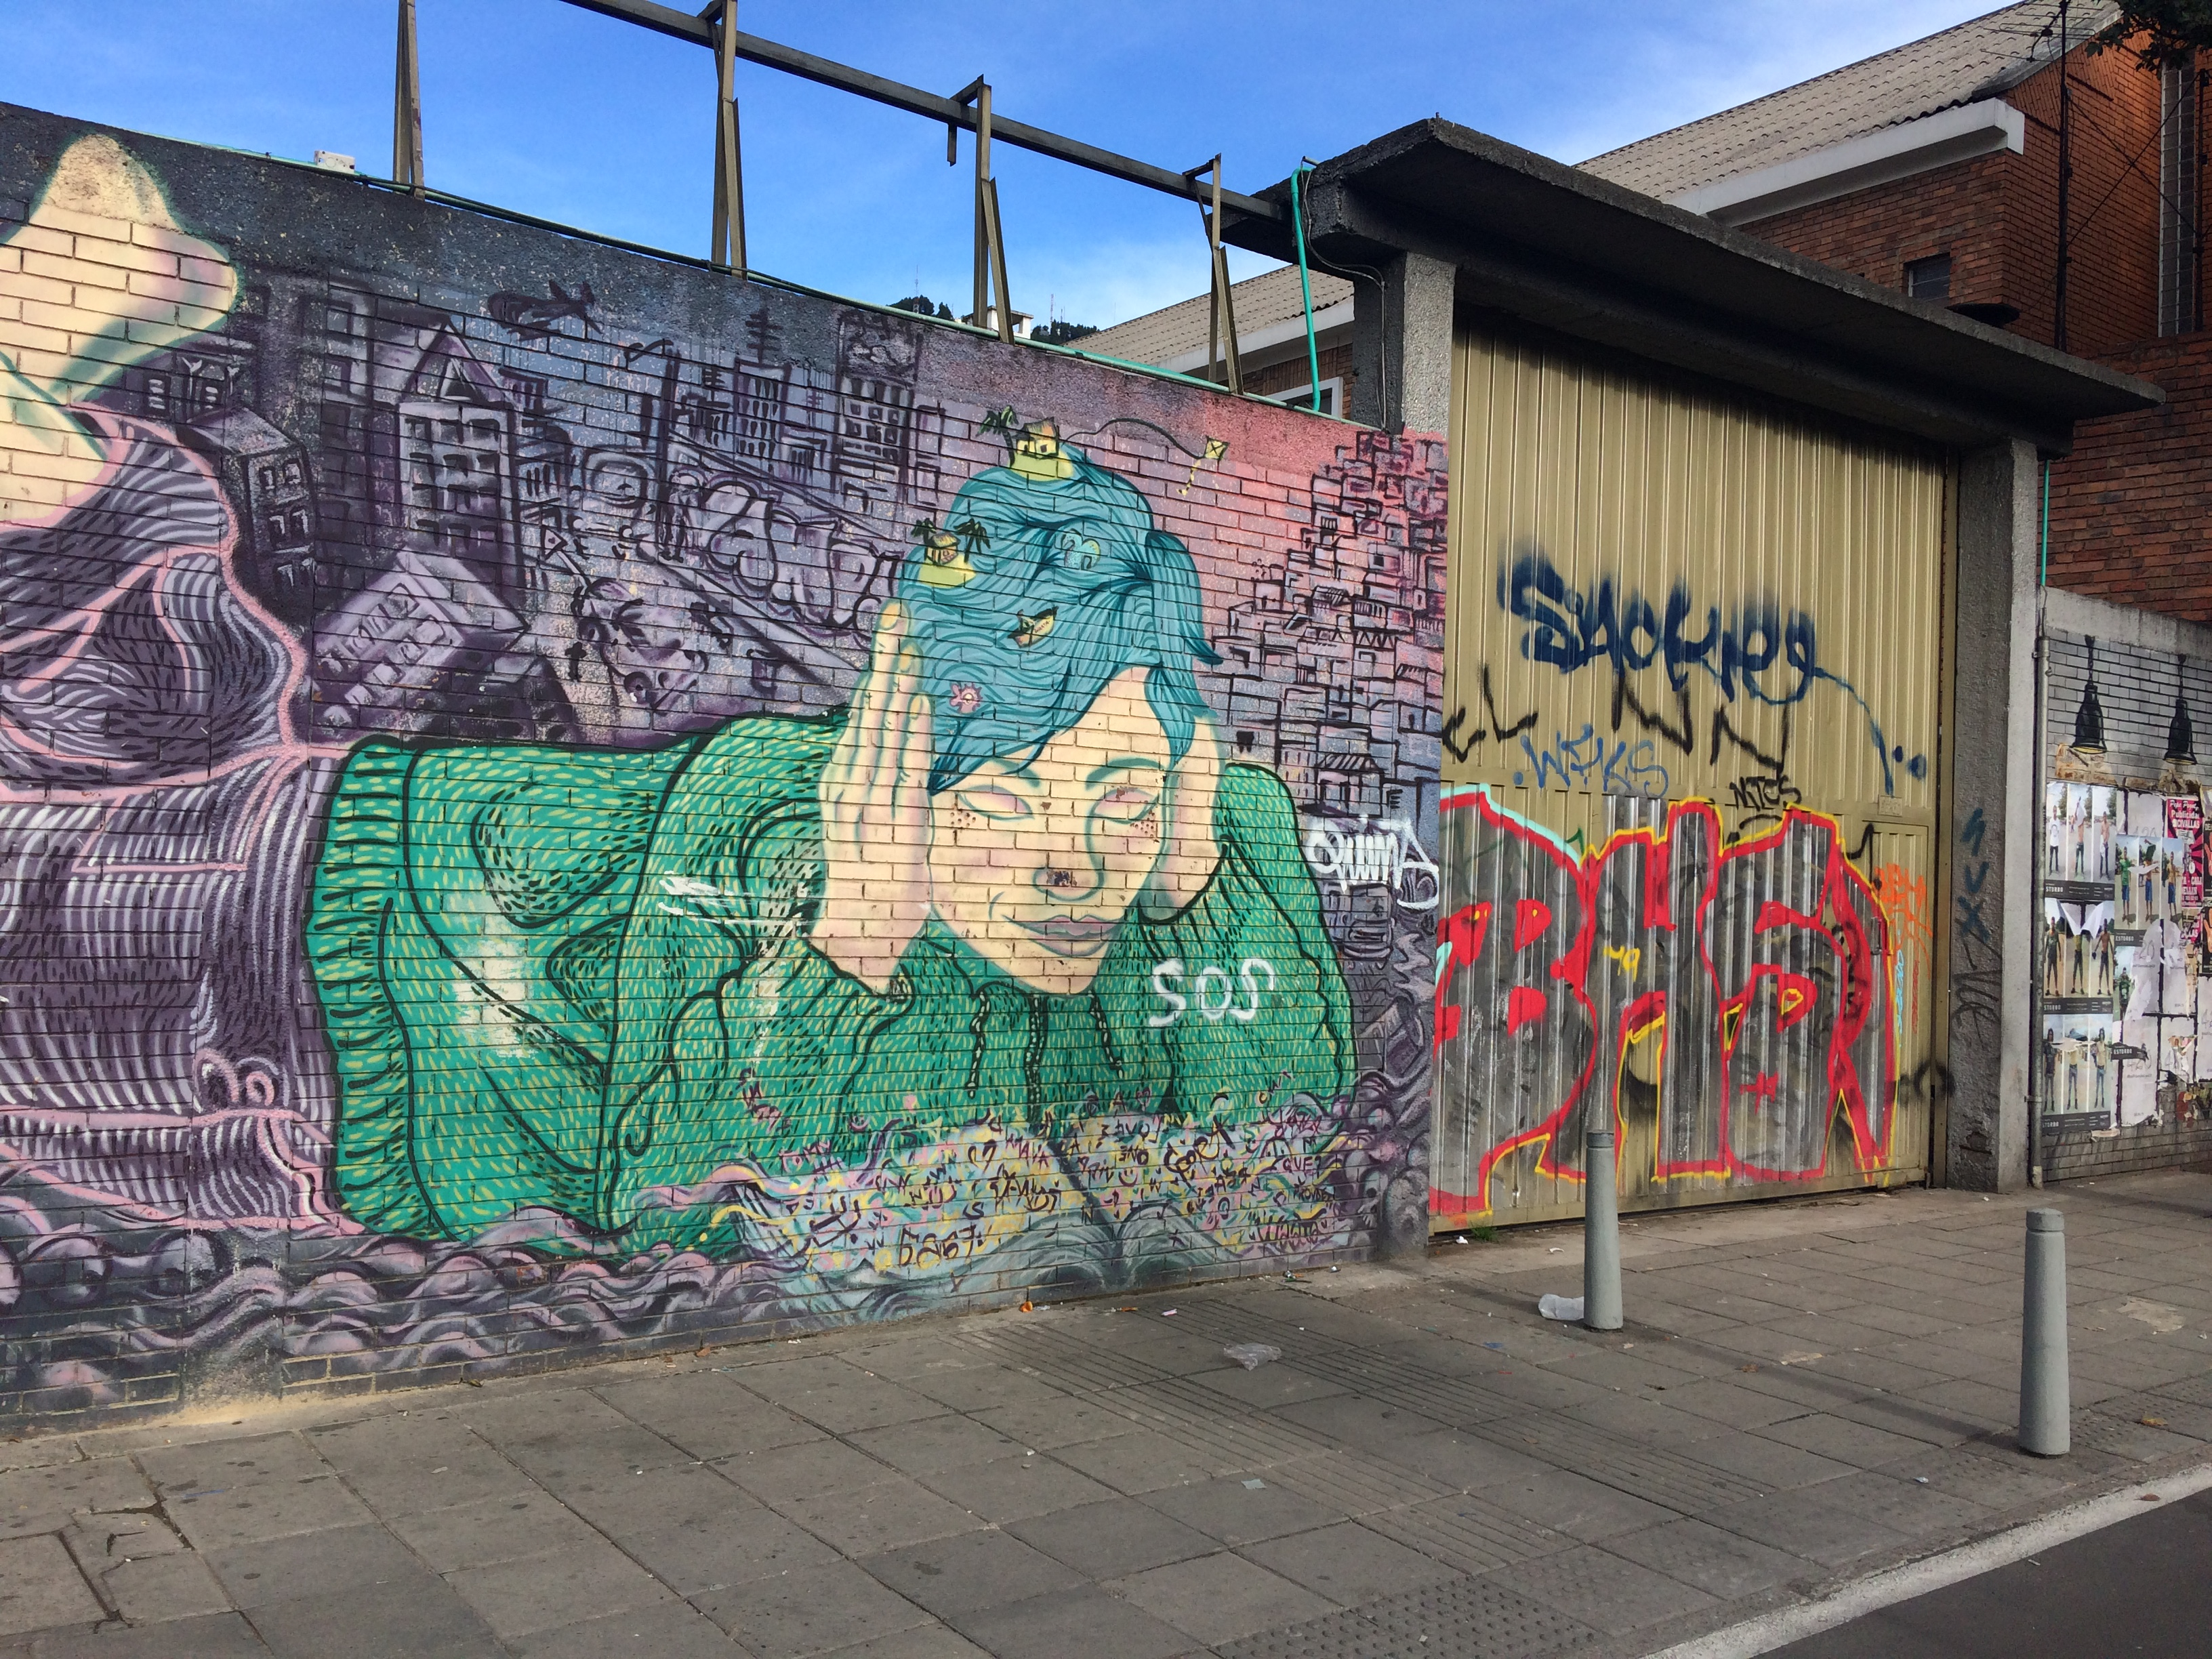
\includegraphics[width=.9\linewidth]{./graffitti/mural_chapinero.JPG} & - composición compleja: & 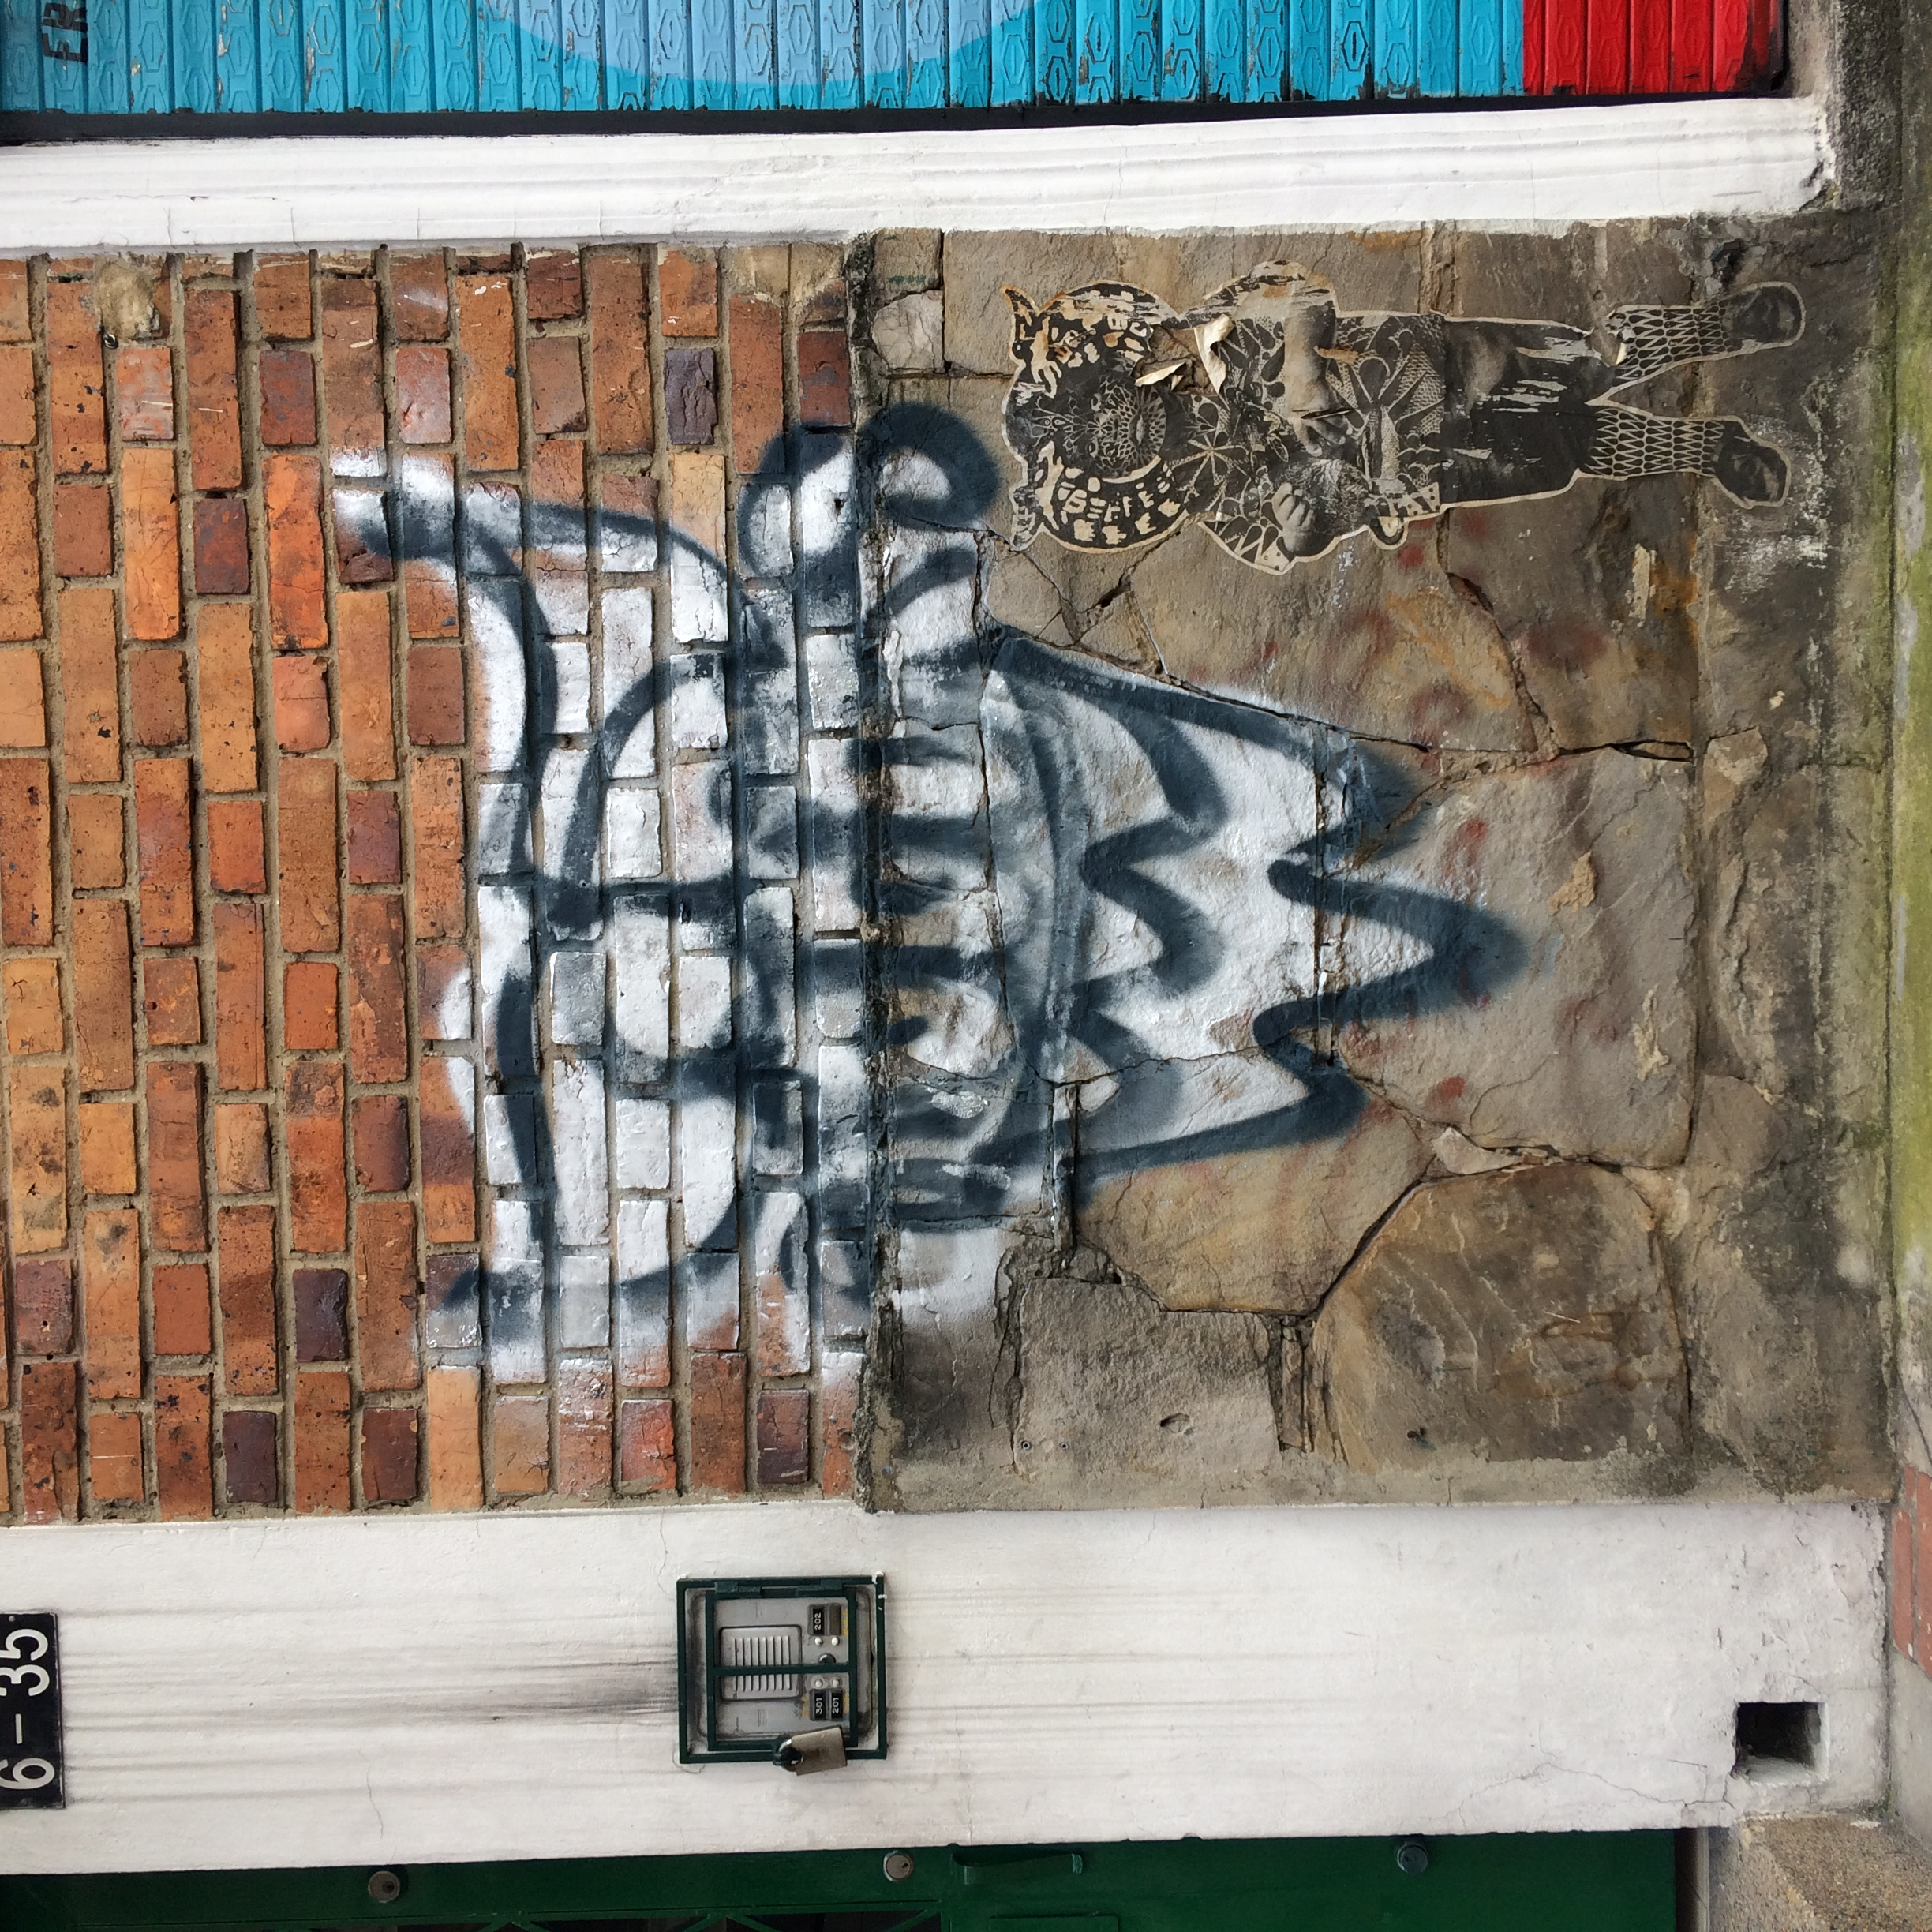
\includegraphics[width=.9\linewidth]{./graffitti/gffti4.JPG} & \\
 & - la ciudad amenaza a joven &  & \\
 & - la "cultura" como salida &  & \\
 & - materiales un poco inferiores &  & \\
 & - intención "muralista" &  & \\
 & - espacio entremezclado con graffiti &  & \\
\hline
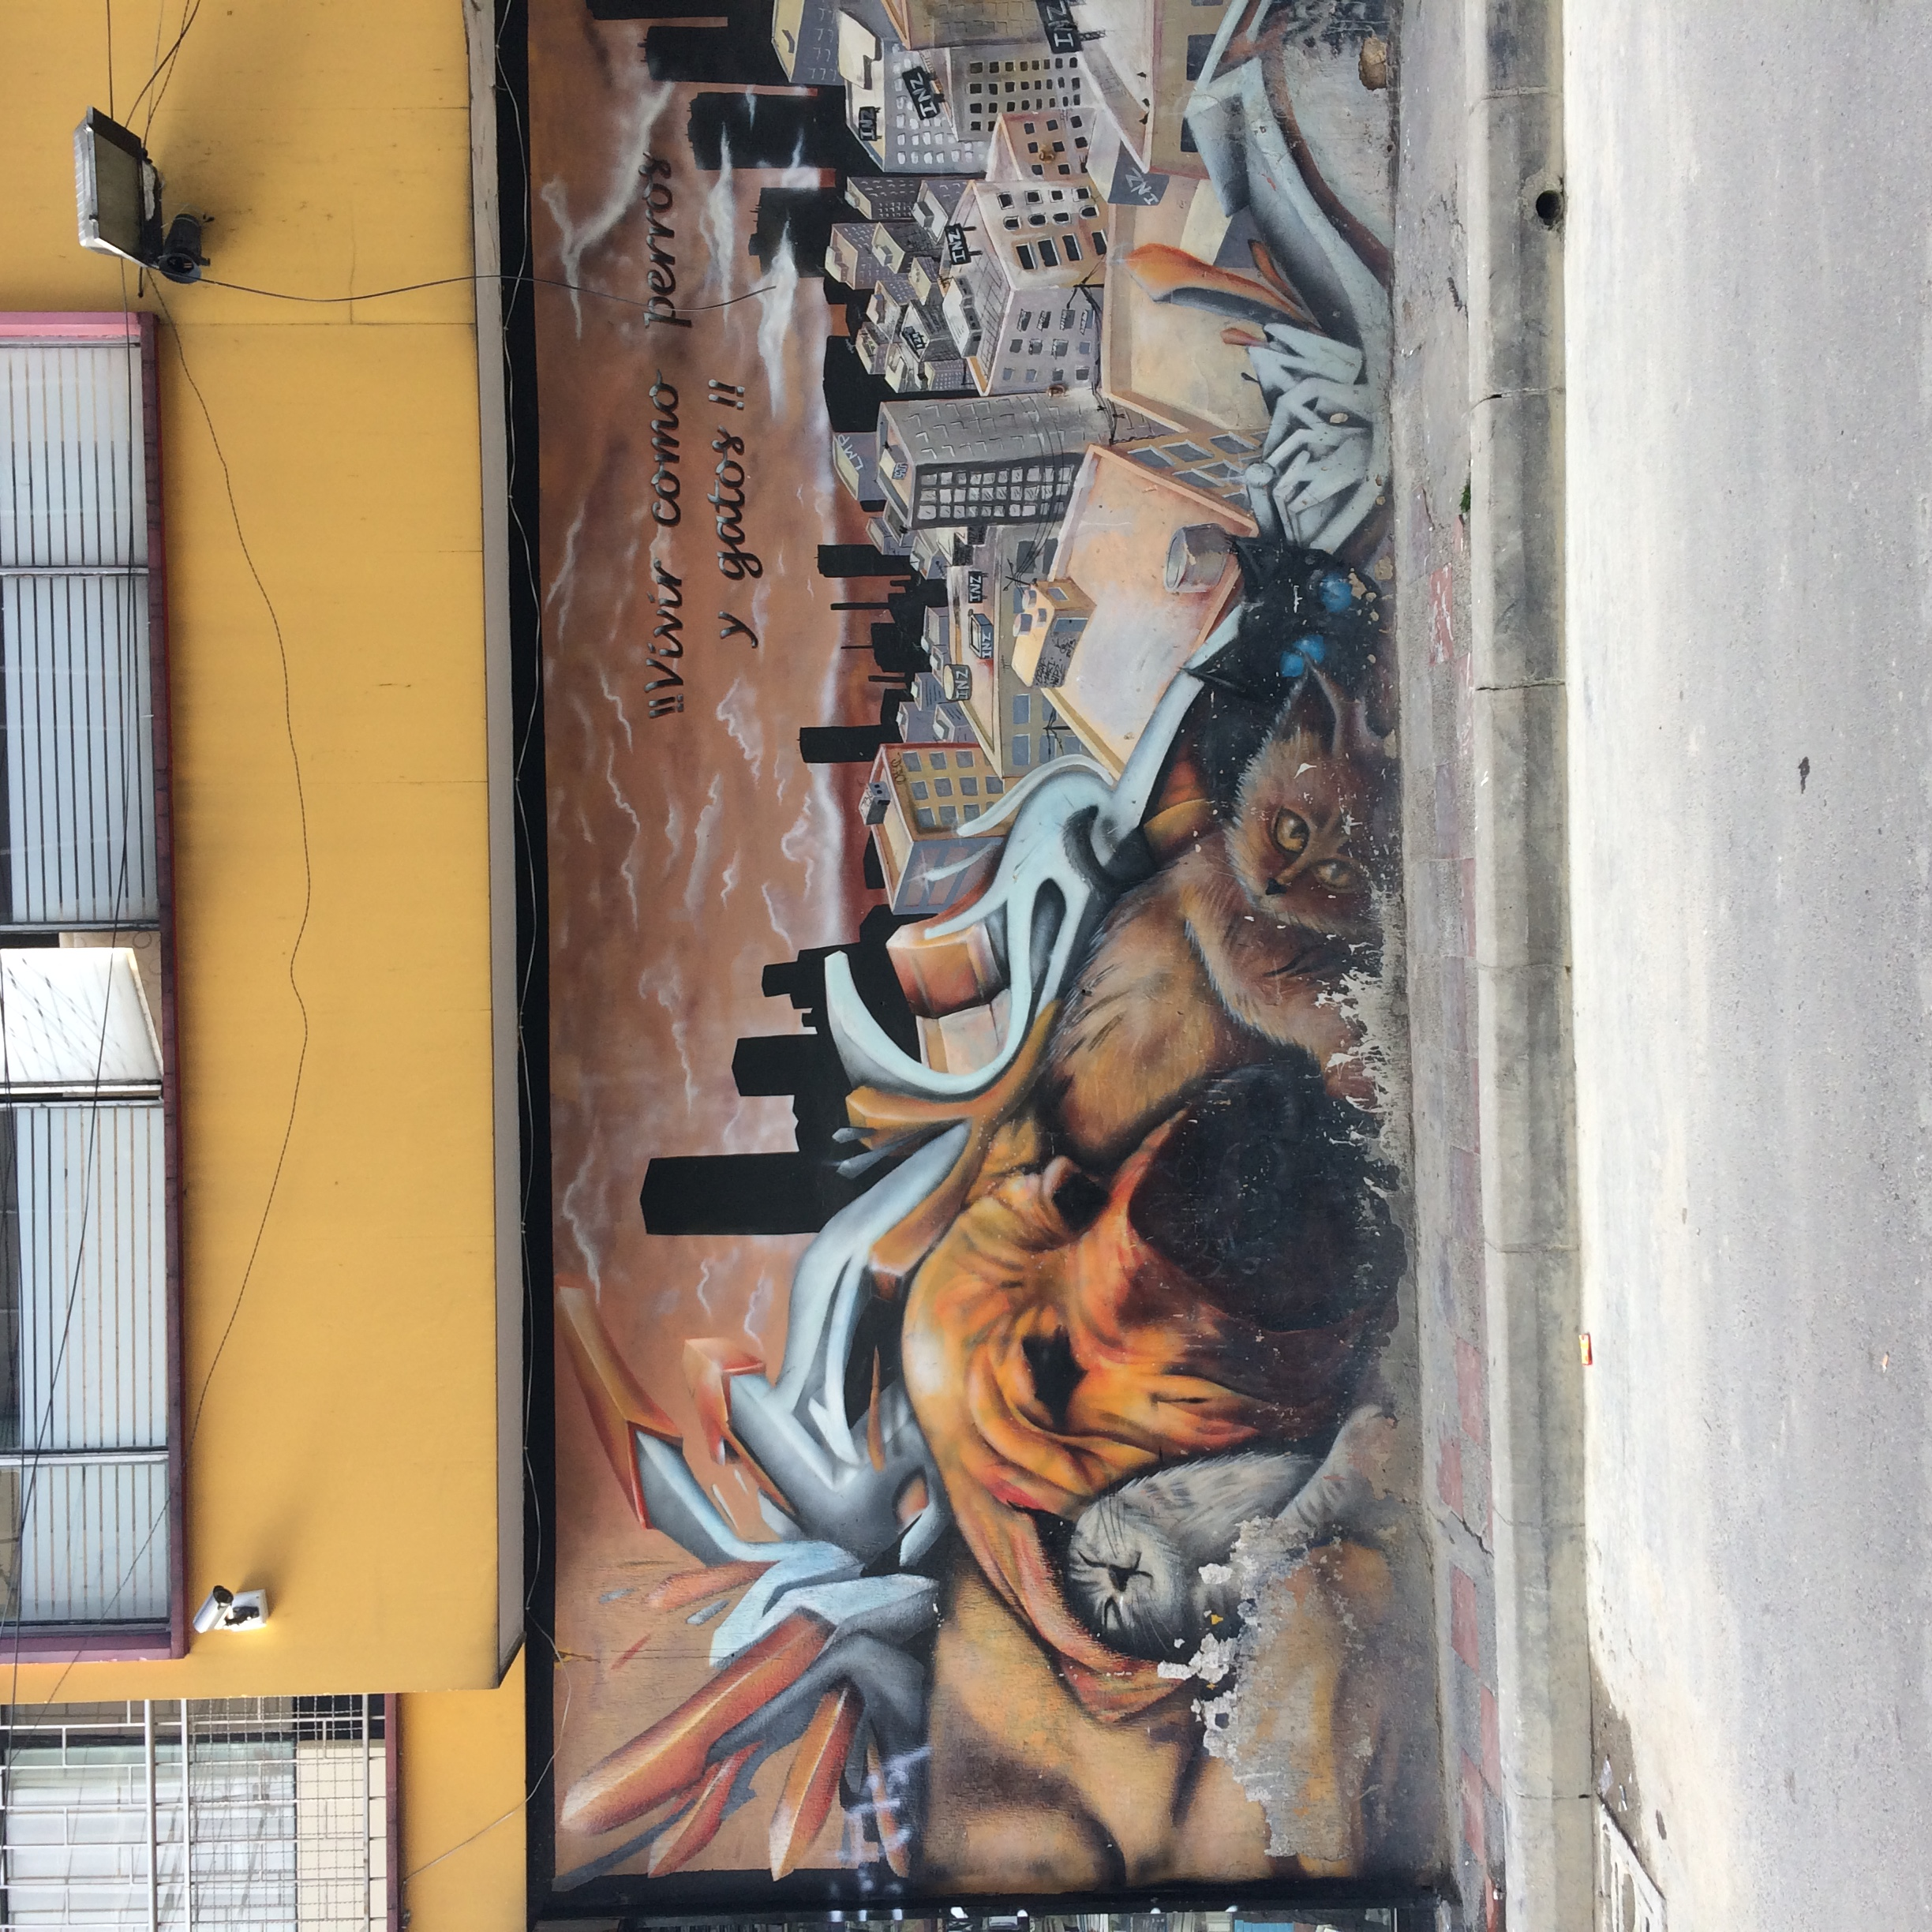
\includegraphics[width=.9\linewidth]{./graffitti/perros.JPG} & - mensaje sobre la ciudad (carga social) & 
\includegraphics[width=.9\linewidth]{./graffitti/gffti5.JPG} & \\
 & - mezcla \emph{lettering} y figuracion &  & \\
 & - firma "Inz" reiteradamente &  & \\
\hline
\end{tabular}
\end{center}
% Emacs 25.3.50.1 (Org mode 8.2.10)
\end{document}